\section{Experiments}
\label{sec:experiments}

% Timetable and planning What will you do with the remainder of my thesis? Give an approximate estimation/timetable for what you will do and when you will be done.

\begin{figure}
    \centering
    \begin{subfigure}{0.45\textwidth}
        \centering
        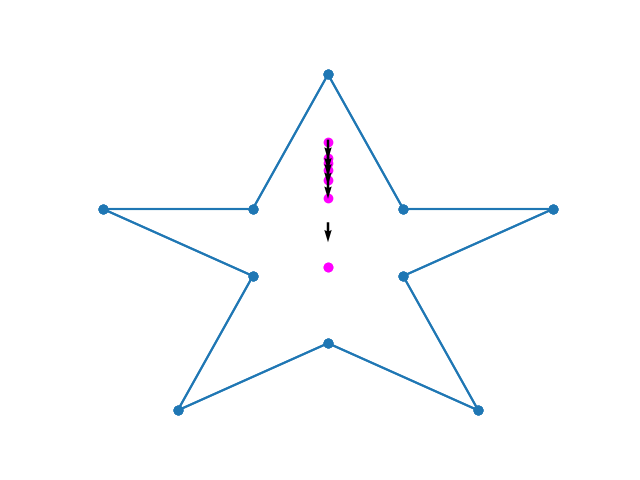
\includegraphics[width = \textwidth]{pentagram_gradient.png}
        \caption{Star polygon gradient example.}
        \label{fig:star_gradient}
    \end{subfigure}
    \begin{subfigure}{0.45\textwidth}
        \centering
        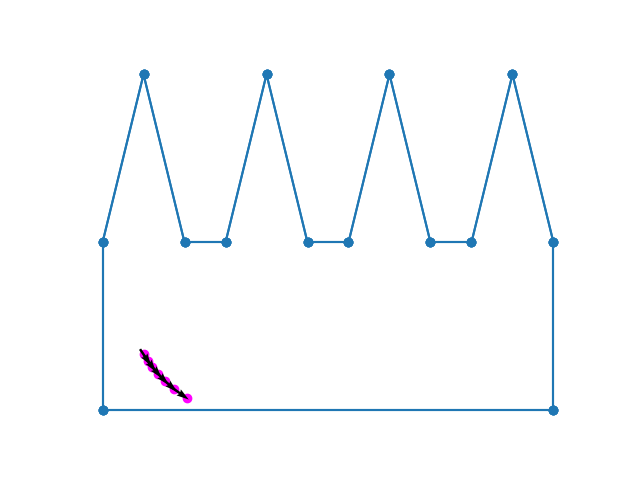
\includegraphics[width = \textwidth]{comb_gradient.png}
        \caption{Comb polygon gradient example.}
        \label{fig:comb_gradient}
    \end{subfigure}
    \begin{subfigure}{0.45\textwidth}
        \centering
        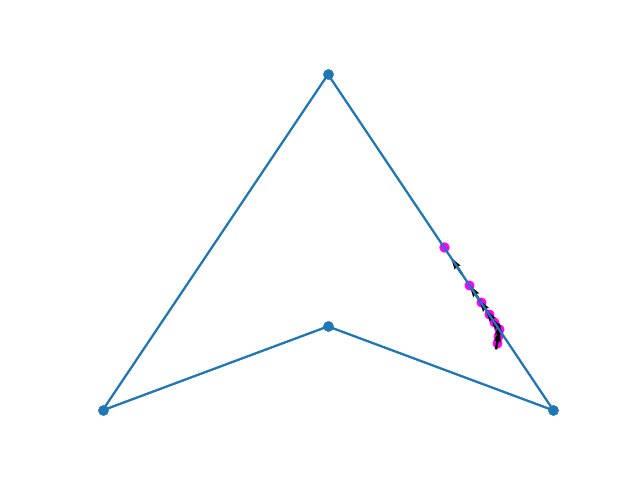
\includegraphics[width = \textwidth]{concave_triangle_gradient.png}
        \caption{Arrowhead polygon gradient example.}
        \label{fig:concave_gradient}
    \end{subfigure}
    \begin{subfigure}{0.45\textwidth}
        \centering
        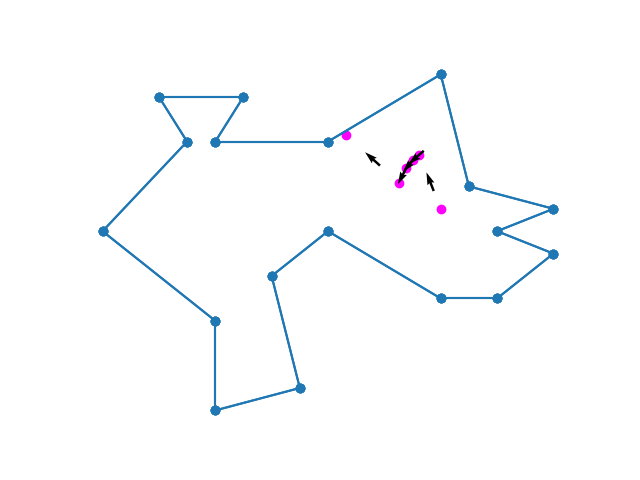
\includegraphics[width = \textwidth]{random_gradient.png}
        \caption{Arbitrary polygon gradient example.}
        \label{fig:random_gradient}
    \end{subfigure}
    \caption{Gradient descent examples on the test polygons.}
\end{figure}